\section[Boosting et AdaBoost]{Boosting et AdaBoost}

\subsection[Introduction]{Introduction}

\begin{frame}{Motivation pour le Boosting}
	\begin{itemize}
		\item On a vu que les Forêts Aléatoires permettent de gérer le compromis biais-variance en utilisant un \textbf{ensemble} de modèles.
		\item L'idée était alors d'entraîner plusieurs arbres avec des réglages agressifs (forte variance) en parallèle (sur des données d'apprentissage bootstrappées) et que l'ensemble permettait de corriger la variance en faisant une moyenne des prédictions.
		\item Le \textbf{Boosting} approche le problème différemment: plusieurs arbres avec des réglages très conservateurs (fort biais) sont entraînés \textbf{séquentiellement} sur des données d'apprentissage et un vote final permet de corriger le biais du modèle.
	\end{itemize}
\end{frame}

\begin{frame}{Idée générale du Boosting}
	L'idée générale du Boosting peut se résumer dans les points suivants:
	\begin{itemize}
		\item On choisit un réglage plutôt conservateur pour un arbre type (en limitant la profondeur maximale entre 1 et 4). Cet arbre a un fort biais. On choisit également le nombre d'arbres à entraîner dans l'ensemble.
		\pause
		\item On entraîne le premier arbre sur les données d'apprentissage. On évalue ses erreurs. Cela déterminera plus tard le nombre de votes que l'arbre aura lors de la prise de décision.
		\pause
		\item On donne une pondération plus importante aux observations mal classifiées par cet arbre, cela constitue les nouvelles données d'apprentissage.
		\pause
		\item On entraîne un second arbre en répétant les étapes du dessus pour le premier arbre.
		\pause
		\item Et ainsi de suite jusqu'à ce que tous les arbres aient été entraînés.
		\pause
		\item Le Boosting fait partie des méthodes \textbf{ensemblistes} en apprentissage automatique.
	\end{itemize}
\end{frame}

\begin{frame}{Les apprenants faibles}
	Dans l'algorithme AdaBoost (Adaptive Boosting), les modèles de base utilisés doivent être très simples. On les qualifie d'\textbf{apprenants faibles} (weak learners).
	\begin{itemize}
		\item En pratique, on utilise souvent un arbre de décision de profondeur 1, appelé \textbf{souche de décision} (decision stump).
		\pause
		\item Une souche ne réalise qu'une seule découpe sur une seule caractéristique.
		\pause
		\item On peut augmenter légèrement la profondeur (ex: 2 à 4) pour permettre au modèle de capter des \textbf{interactions} entre plusieurs variables (ex: pixels croisés d'une image).
		\pause
		\item L'objectif n'est pas que l'arbre soit parfait. La performance viendra de la \textbf{séquence}.
	\end{itemize}
\end{frame}

\subsection[Algorithme]{Algorithme}

\begin{frame}{L'algorithme CART avec des poids}
	Pour que le Boosting fonctionne, notre arbre de décision doit être capable de prêter plus d'attention à certaines observations qu'à d'autres. On introduit un poids $w_i$ pour chaque observation $i$.
	
	\vspace{0.3cm}
	La formule de l'entropie reste inchangée. Cependant, la proportion (probabilité) d'une classe $k$ dans un groupe n'est plus basée sur le comptage des individus, mais sur la \textbf{somme de leurs poids}.
	
	\pause
	\vspace{0.3cm}
	
	Dans un groupe donné, la probabilité d'obtenir la classe $k$ se calcule comme:
	\begin{equation*}
		P(Y = k) = \frac{\sum_{i \in \text{groupe} \mid y^{(i)} = k} w^{(i)}}{\sum_{i \in \text{groupe}} w^{(i)}}
	\end{equation*}
	
	\pause
	
	Cette formule a deux rôles cruciaux :
	\begin{itemize}
		\item \textbf{Pour la découpe :} Elle permet de calculer l'entropie pondérée du nœud.
		\item \textbf{Pour la prédiction :} Si le nœud est une feuille, la classe prédite par l'arbre est celle qui a la probabilité pondérée la plus forte.
	\end{itemize}
\end{frame}

\begin{frame}{Exemple de calcul avec un poids}
	Supposons que nous avons un groupe avec les observations suivantes:
	\begin{table}
		\centering
		\begin{tabular}{|l|c|c|c|c|}
			\hline
			\textbf{Observation} $i$ & 1 & 2 & 3 & 4 \\
			\hline
			\textbf{Classe} $y^{(i)}$ & 0 & 1 & 0 & 1 \\
			\hline
			\textbf{Poids} $w^{(i)}$ & 0.33 & 0.20 & 0.27 & 0.20 \\
			\hline
		\end{tabular}
	\end{table}
	On calcule donc les probabilités suivantes:
	\begin{equation*}
		\begin{cases}
			P(Y = 0) = \frac{0.33 + 0.27}{1} = 0.6 \\
			P(Y = 1) = \frac{0.20 + 0.20}{1} = 0.4
		\end{cases}
	\end{equation*}
	L'entropie $H(Y)$ se calcule comme suit:
	\begin{equation*}
		\begin{aligned}
			H(Y) 
			&= \sum_{k=0}^2 P(Y = k) I(Y = k) \\
			&= - P(Y = 0) \ln P(Y = 0) - P(Y = 1) \ln P(Y = 1) \\
			&= - 0.6 \ln 0.6 - 0.4 \ln 0.4 \\
			&\approx 0.673
		\end{aligned}
	\end{equation*}
\end{frame}

\begin{frame}{Initialisation et erreur}
	Pour un problème de classification à $K$ classes, nous utiliserons la généralisation multiclasse d'AdaBoost appelée \textbf{SAMME}:
	\begin{enumerate}
		\item On initialise toutes les observations au même poids: $w_1^{(i)} = \frac{1}{n}$.
		\pause
		\item Pour chaque arbre $m$ de $1$ à $M$, on entraîne l'arbre $m$ sur les données pondérées. On calcule ensuite son \textbf{erreur pondérée} $\epsilon_m \in [0, 1]$, qui est la somme des poids des observations qu'il a mal classées:
		\begin{equation*}
			\epsilon_m = \frac{\sum_{i=1}^n w_m^{(i)} \mathds{1}(\hat{f}_m(x^{(i)}) \neq y^{(i)})}{\sum_{i=1}^n w_m^{(i)}}
		\end{equation*}
		Où $\hat{f}_m(x^{(i)})$ est la prédiction de l'arbre $m$ pour l'observation $i$ et $\mathds{1}$ est la fonction indicatrice (vaut $1$ si la condition est vraie, $0$ sinon).
		\pause
		\item On vérifie un critère d'arrêt. Si $\epsilon_m \ge (K - 1)/ K$ le boosting s'arrête prématurément (on aura moins de M arbres). Parce que l'arbre fait moins bien qu'une décision purement arbitraire.
	\end{enumerate}
\end{frame}

\begin{frame}{Calcul du poids de vote de l'arbre}
	Une fois l'erreur $\epsilon_m$ calculée, on détermine l'importance ou le \textbf{poids de vote} de l'arbre $m$, noté $\alpha_m \in \R^+$. Plus l'arbre est précis, plus son poids sera grand:
	
	\begin{equation*}
		\alpha_m = \nu \left[\ln \left( \frac{1 - \epsilon_m}{\epsilon_m + \delta} \right) + \ln(K - 1)\right]
	\end{equation*}
	
	\pause
	\vspace{0.3cm}
	Le terme $\ln(K - 1)$ garantit que le poids de l'arbre sera positif tant que son erreur $\epsilon_m$ est inférieure à $(K-1)/K$. Le terme $\delta$ est une faible valeur numérique pour éviter une division par zéro (typiquement $10^{-8}$). Enfin, $\nu$ est un \textbf{taux d'apprentissage}. Il permet de moduler les variations de poids des observations (voir plus loin). Une valeur typique est $\nu = 1$, une valeur plus petite nécessitera davantage d'arbres. C'est donc un hyper-paramètre d'AdaBoost.
\end{frame}

\begin{frame}{Exemple de calcul de poids de vote}
	Dans notre problème MNIST nous avons $K = 10$:
	\begin{itemize}
		\item Un algorithme prenant une décision arbitraire a donc 10\% de chance de donner une bonne réponse. Et a donc 90\% de chance de donner une mauvaise réponse. Donc si $\epsilon_m \ge 0.9$ l'arbre est moins bon qu'une décision arbitraire. On a donc un arrêt prématuré.
		\item Un algorithme avec un taux d'erreur $\epsilon_m = 0.89$ est mauvais mais meilleur qu'une décision arbitraire. En prenant $\nu = 1$:
		\begin{equation*}
			\begin{aligned}
				\alpha_m 
				&= \ln \left( \frac{1 - \epsilon_m}{\epsilon_m + \delta} \right) + \ln(K - 1) \\
				&= \ln \frac{1 - 0.89}{0.89} + \ln(10 - 1) \\
				&\approx 0.106
			\end{aligned}
		\end{equation*}
		Le terme $\ln(K - 1)$ garantit un poids de vote positif lorsque l'arbre est meilleur qu'une décision arbitraire.
	\end{itemize}
\end{frame}

\begin{frame}{Mise à jour des poids des observations}
	C'est ici que l'algorithme s'adapte (Boosting adaptatif). On met à jour le poids de chaque observation pour le passage à l'arbre suivant $m+1$ pour l'observation $i$:
	
	\begin{equation*}
		w_{m+1}^{(i)} = w_m^{(i)} \exp\left(\alpha_m \mathds{1}(\hat{f}_m(x^{(i)}) \neq y^{(i)})\right)
	\end{equation*}
	
	\pause
	\begin{itemize}
		\item Si l'arbre a prédit correctement: $\mathds{1}(\hat{f}_m(x^{(i)}) \neq y^{(i)}) = 0$, donc $\exp(0) = 1$. Le poids \textbf{ne change pas}.
		\item Si l'arbre s'est trompé: $\mathds{1}(\hat{f}_m(x^{(i)}) \neq y^{(i)}) = 1$. Le poids est multiplié par $\exp(\alpha_m)$. Il \textbf{augmente} donc d'autant plus fortement que l'arbre a obtenu un taux d'erreur $\epsilon_m$ faible !
	\end{itemize}
	
	\vspace{0.3cm}
	Enfin, on \textbf{normalise} tous les poids $w_{m+1}^{(i)}$ pour que leur somme vaille à nouveau $1$ avant d'entraîner le prochain arbre.
\end{frame}

\begin{frame}{Prise de décision finale (Le vote)}
	Une fois les $M$ arbres entraînés, pour prédire la classe d'une nouvelle observation $x$, l'ensemble organise un vote pondéré.
	
	\vspace{0.5cm}
	On fait la somme des poids $\alpha_m$ des arbres qui ont voté pour chaque classe $k$. Pour des données d'inférence $x_i$, la classe gagnante $\hat{f}(x_i)$ est celle qui obtient le score cumulé le plus élevé:	
	\begin{equation*}
		\hat{f}(x_i) = \argmax{k} \sum_{m=1}^M \alpha_m \mathds{1}(\hat{f}_m(x_i) = k)
	\end{equation*}
\end{frame}

\begin{frame}{Calcul des probabilités}
	Certaines métriques (comme la surface sous la courbe ROC) nécessitent de prédire des \textbf{probabilités} plutôt que des classes fermes.
	
	\vspace{0.5cm}
	Dans AdaBoost, la probabilité d'une classe $k$ s'obtient simplement en calculant le \textbf{pourcentage des voix} (les poids de vote) récoltées par cette classe par rapport à la somme des voix de tous les arbres:
	
	\begin{equation*}
		P(Y = k \mid x_i) = \frac{\sum_{m=1}^M \alpha_m \mathds{1}(\hat{f}_m(x_i) = k)}{\sum_{m=1}^M \alpha_m}
	\end{equation*}

\end{frame}

\subsection[Cas d'étude]{Cas d'étude}

\begin{frame}{Simplification et algorithmes}
	Nous entraînerons un AdaBoost avec un arbre de décision sur les données MNIST en utilisant une simplification des données obtenue par analyse en composantes principales.
	
	\vspace{0.5cm}
	
	Les algorithmes de Scikit-Learn que nous utiliserons:
	\begin{itemize}
		\item \href{https://scikit-learn.org/stable/modules/generated/sklearn.decomposition.PCA.html}{\texttt{sklearn.decomposition.PCA}}
		\item \href{https://scikit-learn.org/stable/modules/generated/sklearn.tree.DecisionTreeClassifier.html}{\texttt{sklearn.tree.DecisionTreeClassifier}}
		\item \href{https://scikit-learn.org/stable/modules/generated/sklearn.ensemble.AdaBoostClassifier.html}{\texttt{sklearn.ensemble.AdaBoostClassifier}}
	\end{itemize}
\end{frame}

\begin{frame}{Exemples de résultats}
	Voici un résultat obtenu sur le dataset MNIST en utilisant AdaBoost combiné à un arbre de décision:
	\begin{columns}
		\begin{column}{0.5\textwidth}
			\begin{figure}
				\centering
				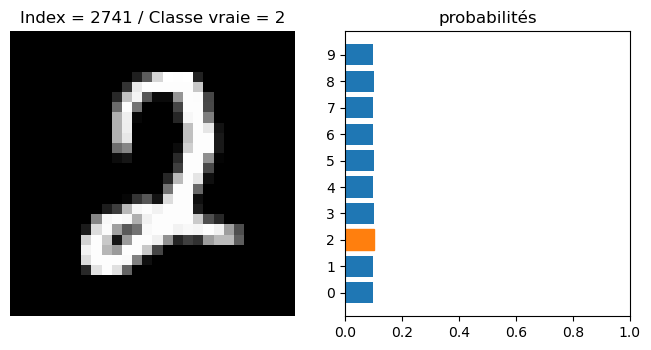
\includegraphics[width=1.0\linewidth]{Images/MNIST_3}
				\label{fig:MNIST_3}
			\end{figure}			
		\end{column}
		\begin{column}{0.5\textwidth}
			\begin{figure}
				\centering
				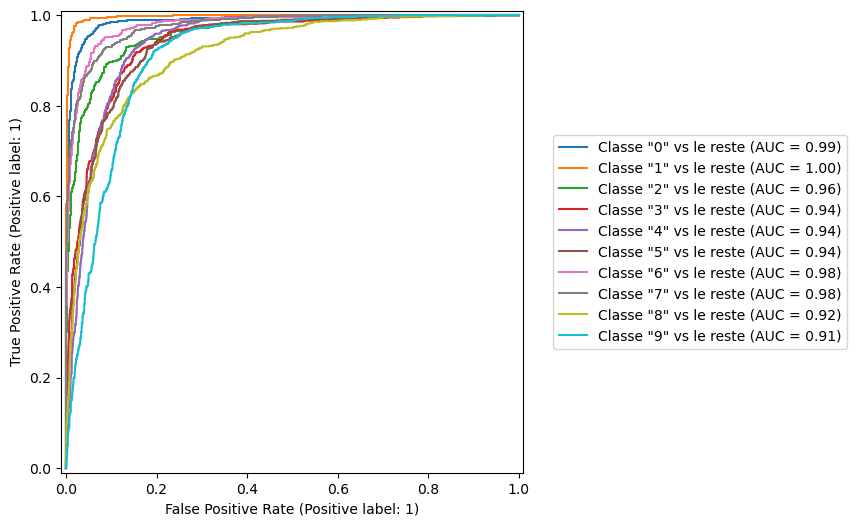
\includegraphics[width=1.0\linewidth]{Images/MNIST_4}
				\label{fig:MNIST_4}
			\end{figure}			
		\end{column}
	\end{columns}
	Attention, AdaBoost ne cherche pas à maximiser la probabilité calculée pour la classe vraie, juste à la rendre marginalement plus grande que pour les autres classes. La simple vue des courbes ROC ne permet pas de se rendre compte de ce comportement.
\end{frame}

\subsection[Synthèse]{Synthèse}

\begin{frame}{AdaBoost (SAMME)}
	\begin{figure}
		\centering
		\resizebox{\textwidth}{!}{
			\begin{tikzpicture}[
				>=stealth,
				node distance=1.2cm and 1.5cm,
				data/.style={circle, draw=black, fill=blue!10, minimum size=1.8cm, align=center, font=\footnotesize},
				tree/.style={rectangle, draw=black, fill=red!15, minimum width=2cm, minimum height=1cm, align=center, font=\footnotesize},
				agg/.style={rectangle, rounded corners, draw=black, fill=yellow!20, minimum width=4cm, minimum height=1cm, align=center},
				arrow/.style={thick, ->}
				]
				
				% Noeuds de donnees
				\node[data] (D1) {$\mathcal{D}$\\$w_1^{(i)}$ égaux};
				\node[data, fill=purple!20] (D2) [right=2cm of D1] {$\mathcal{D}$\\$w_2^{(i)}$ modifiés};
				\node (Dots) [right=1.2cm of D2] {\Large \dots};
				\node[data, fill=red!30] (DM) [right=1.2cm of Dots] {$\mathcal{D}$\\$w_M^{(i)}$ modifiés};
				
				% Noeuds d'arbres
				\node[tree] (T1) [below=0.4cm of D1] {Arbre 1\\(Souche)};
				\node[tree] (T2) [below=0.4cm of D2] {Arbre 2\\(Souche)};
				\node[tree] (TM) [below=0.4cm of DM] {Arbre $M$\\(Souche)};
				
				% Poids alpha
				\node[font=\footnotesize\color{red!70!black}] (A1) [below=0.05cm of T1, xshift=-0.8cm] {Poids: $\alpha_1$};
				\node[font=\footnotesize\color{red!70!black}] (A2) [below=0.05cm of T2, xshift=-0.8cm] {Poids: $\alpha_2$};
				\node[font=\footnotesize\color{red!70!black}] (AM) [below=0.05cm of TM, xshift=-0.8cm] {Poids: $\alpha_M$};
				
				% Noeud Vote
				\node[agg] (Vote) [below=2.0cm of D2] {Vote Pondéré\\$\hat{f}(x_i) = \argmax{k} \sum_{m=1}^M \alpha_m \mathds{1}(\hat{f}_m(x_i) = k)$};
				\node (Out) [below=0.4cm of Vote] {\textbf{Prédiction}};
				
				% Fleches horizontales (mise a jour)
				\draw[arrow] (D1) -- (T1);
				\draw[arrow] (T1.east) -- node[above, sloped, font=\scriptsize] {Erreur $\epsilon_1$} node[below, sloped, font=\scriptsize] {Maj $w_2^{(i)}$} (D2.south west);
				\draw[arrow] (D2) -- (T2);
				\draw[arrow] (T2.east) -- node[above, sloped, font=\scriptsize] {Erreur $\epsilon_2$} (Dots.south west);
				\draw[arrow] (DM) -- (TM);
				
				% Fleches vers le vote
				\draw[arrow, dashed] (T1.south) |- (Vote.west);
				\draw[arrow, dashed] (T2.south) -- (Vote.north);
				\draw[arrow, dashed] (TM.south) |- (Vote.east);
				
				\draw[arrow] (Vote) -- (Out);
				
			\end{tikzpicture}
		}
	\end{figure}
	Architecture \textbf{séquentielle}. On réduit le \textbf{biais} en chaînant des modèles simples.
\end{frame}
